\section{Inlining blocks}

The blocks which have only one incoming block and are not blocks that appear after a recursive call can be inlined in
the incoming block. This is accomplished by marking the blocks that can be inlined first and then visiting the blocks
that cannot be inlined in order to generate the new blocks.

An example of this pass is provided in \labelindexref{Figure}{img:inline-blocks}. The blocks with \code{id}s \code{1},
\code{3}, \code{4} and \code{6} have been inlined where the jump to them takes place, thus significantly reducing the
number of blocks.

\begin{figure}[htb]
    \makebox[\linewidth][c]{%
    \begin{subfigure}[b]{.6\textwidth}
        \centering
        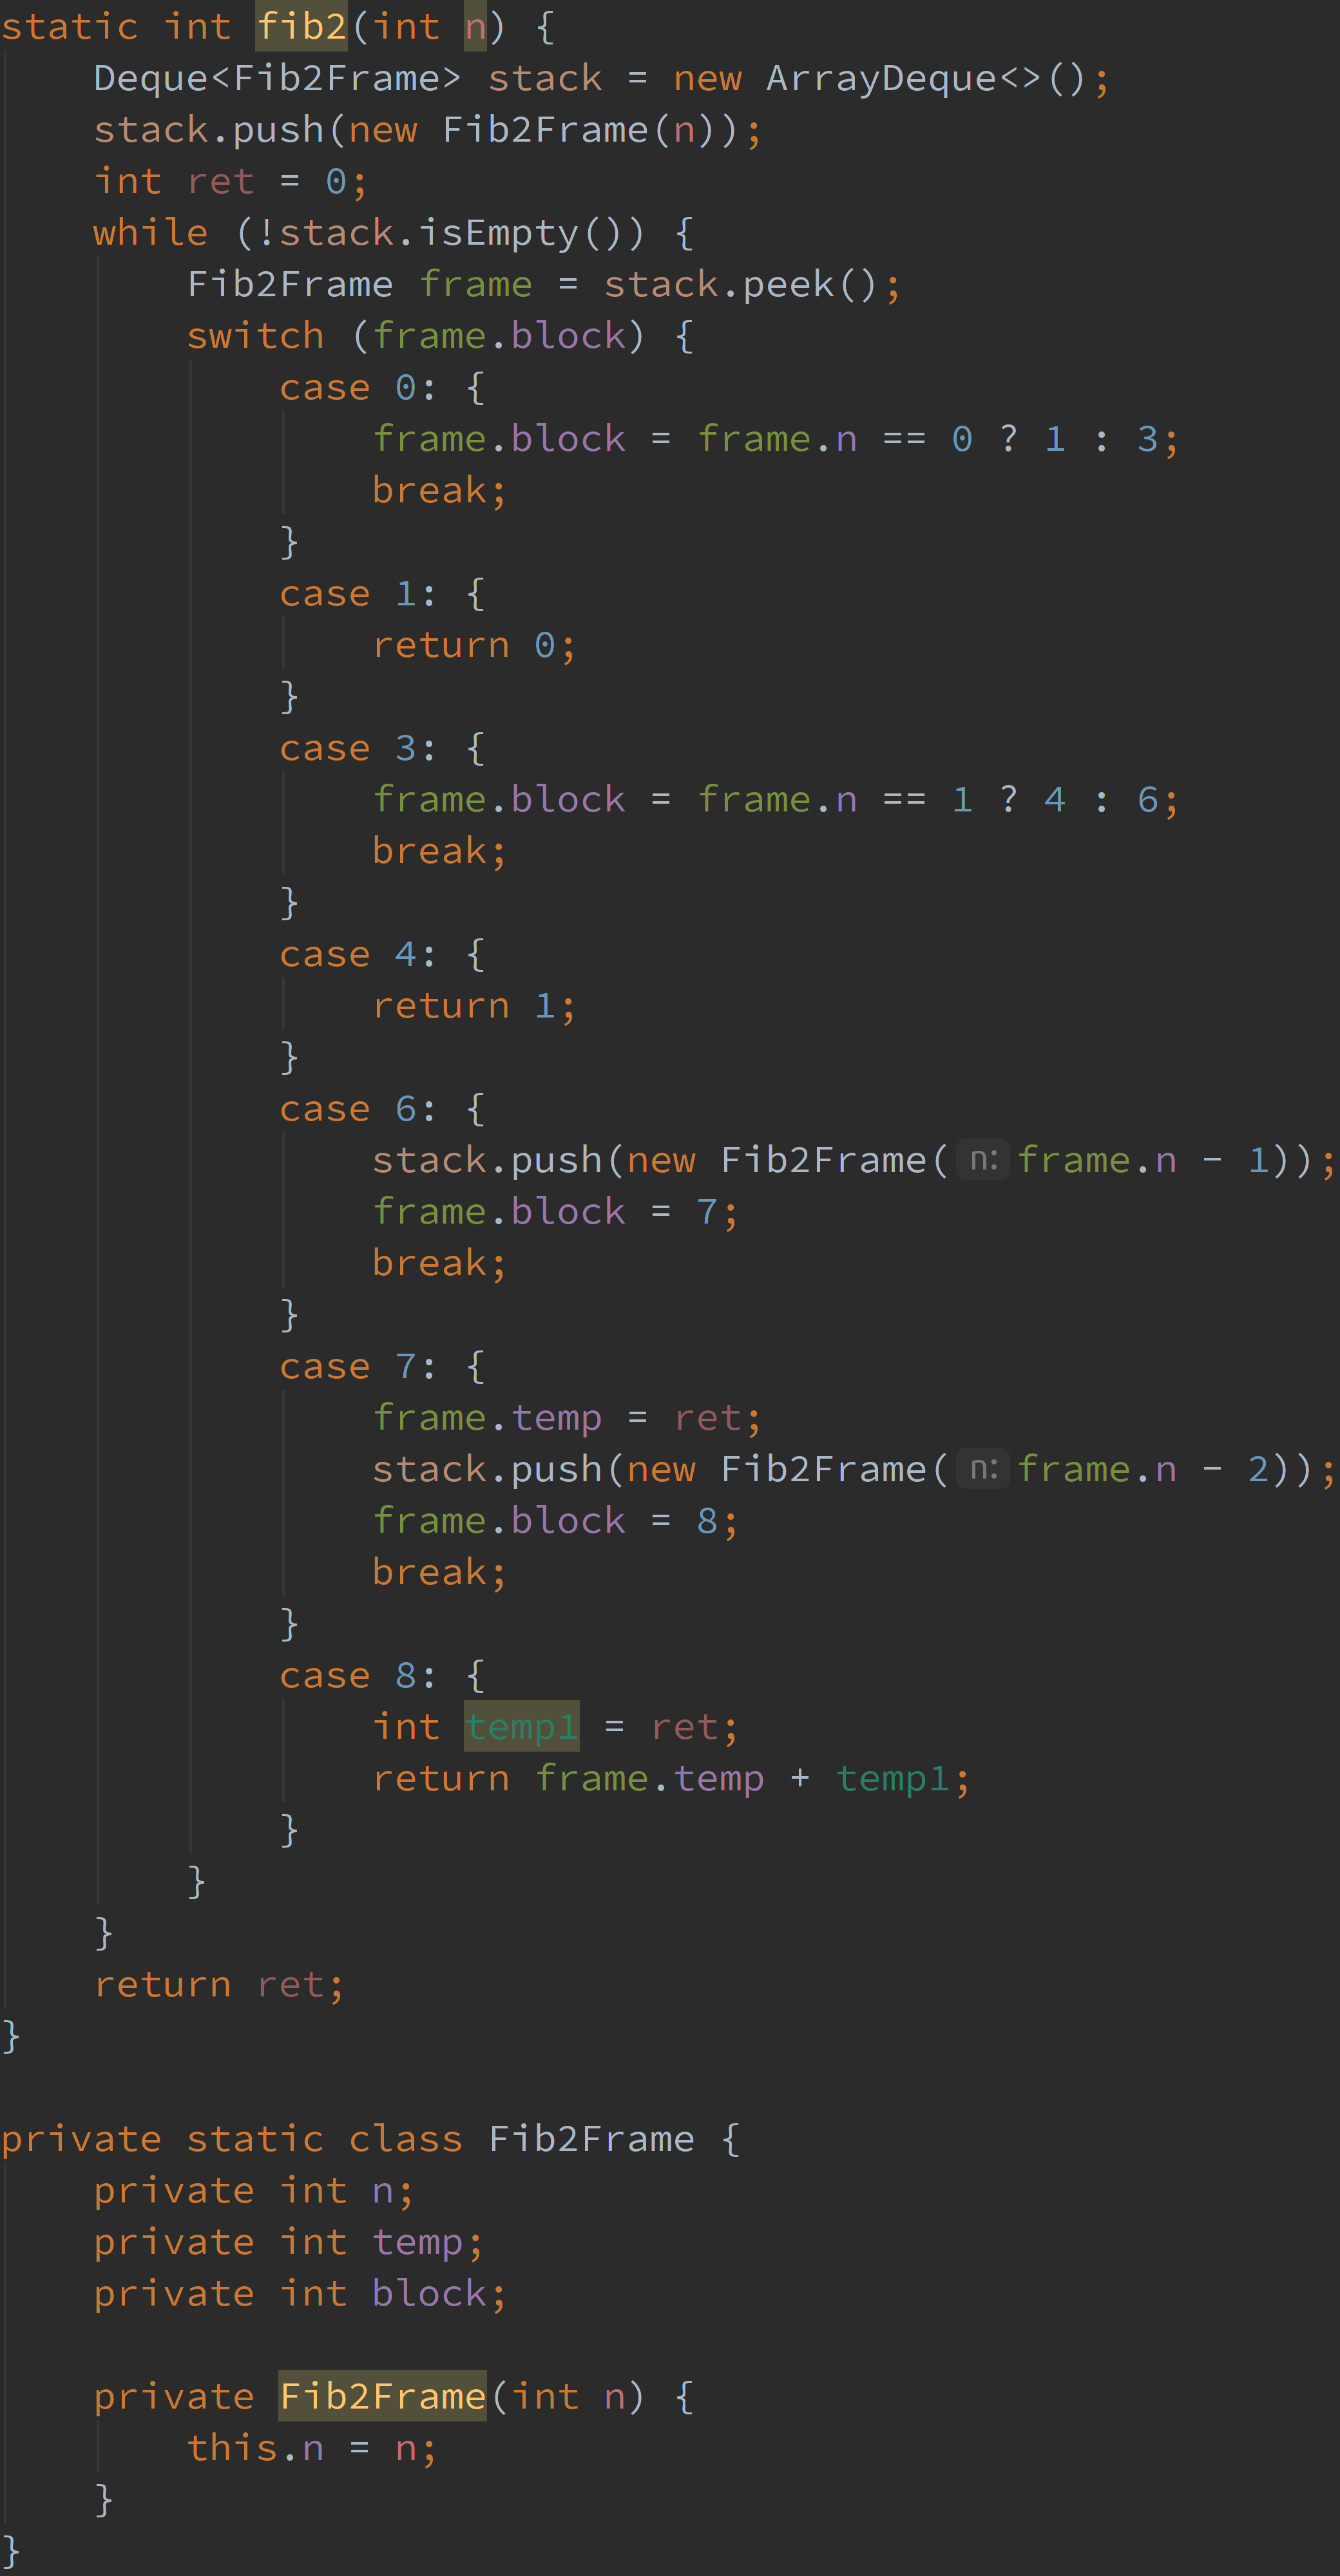
\includegraphics[height=5in]{src/img/inline-blocks-before.png}
        \caption{Before}
    \end{subfigure}%
    \begin{subfigure}[b]{.6\textwidth}
        \centering
        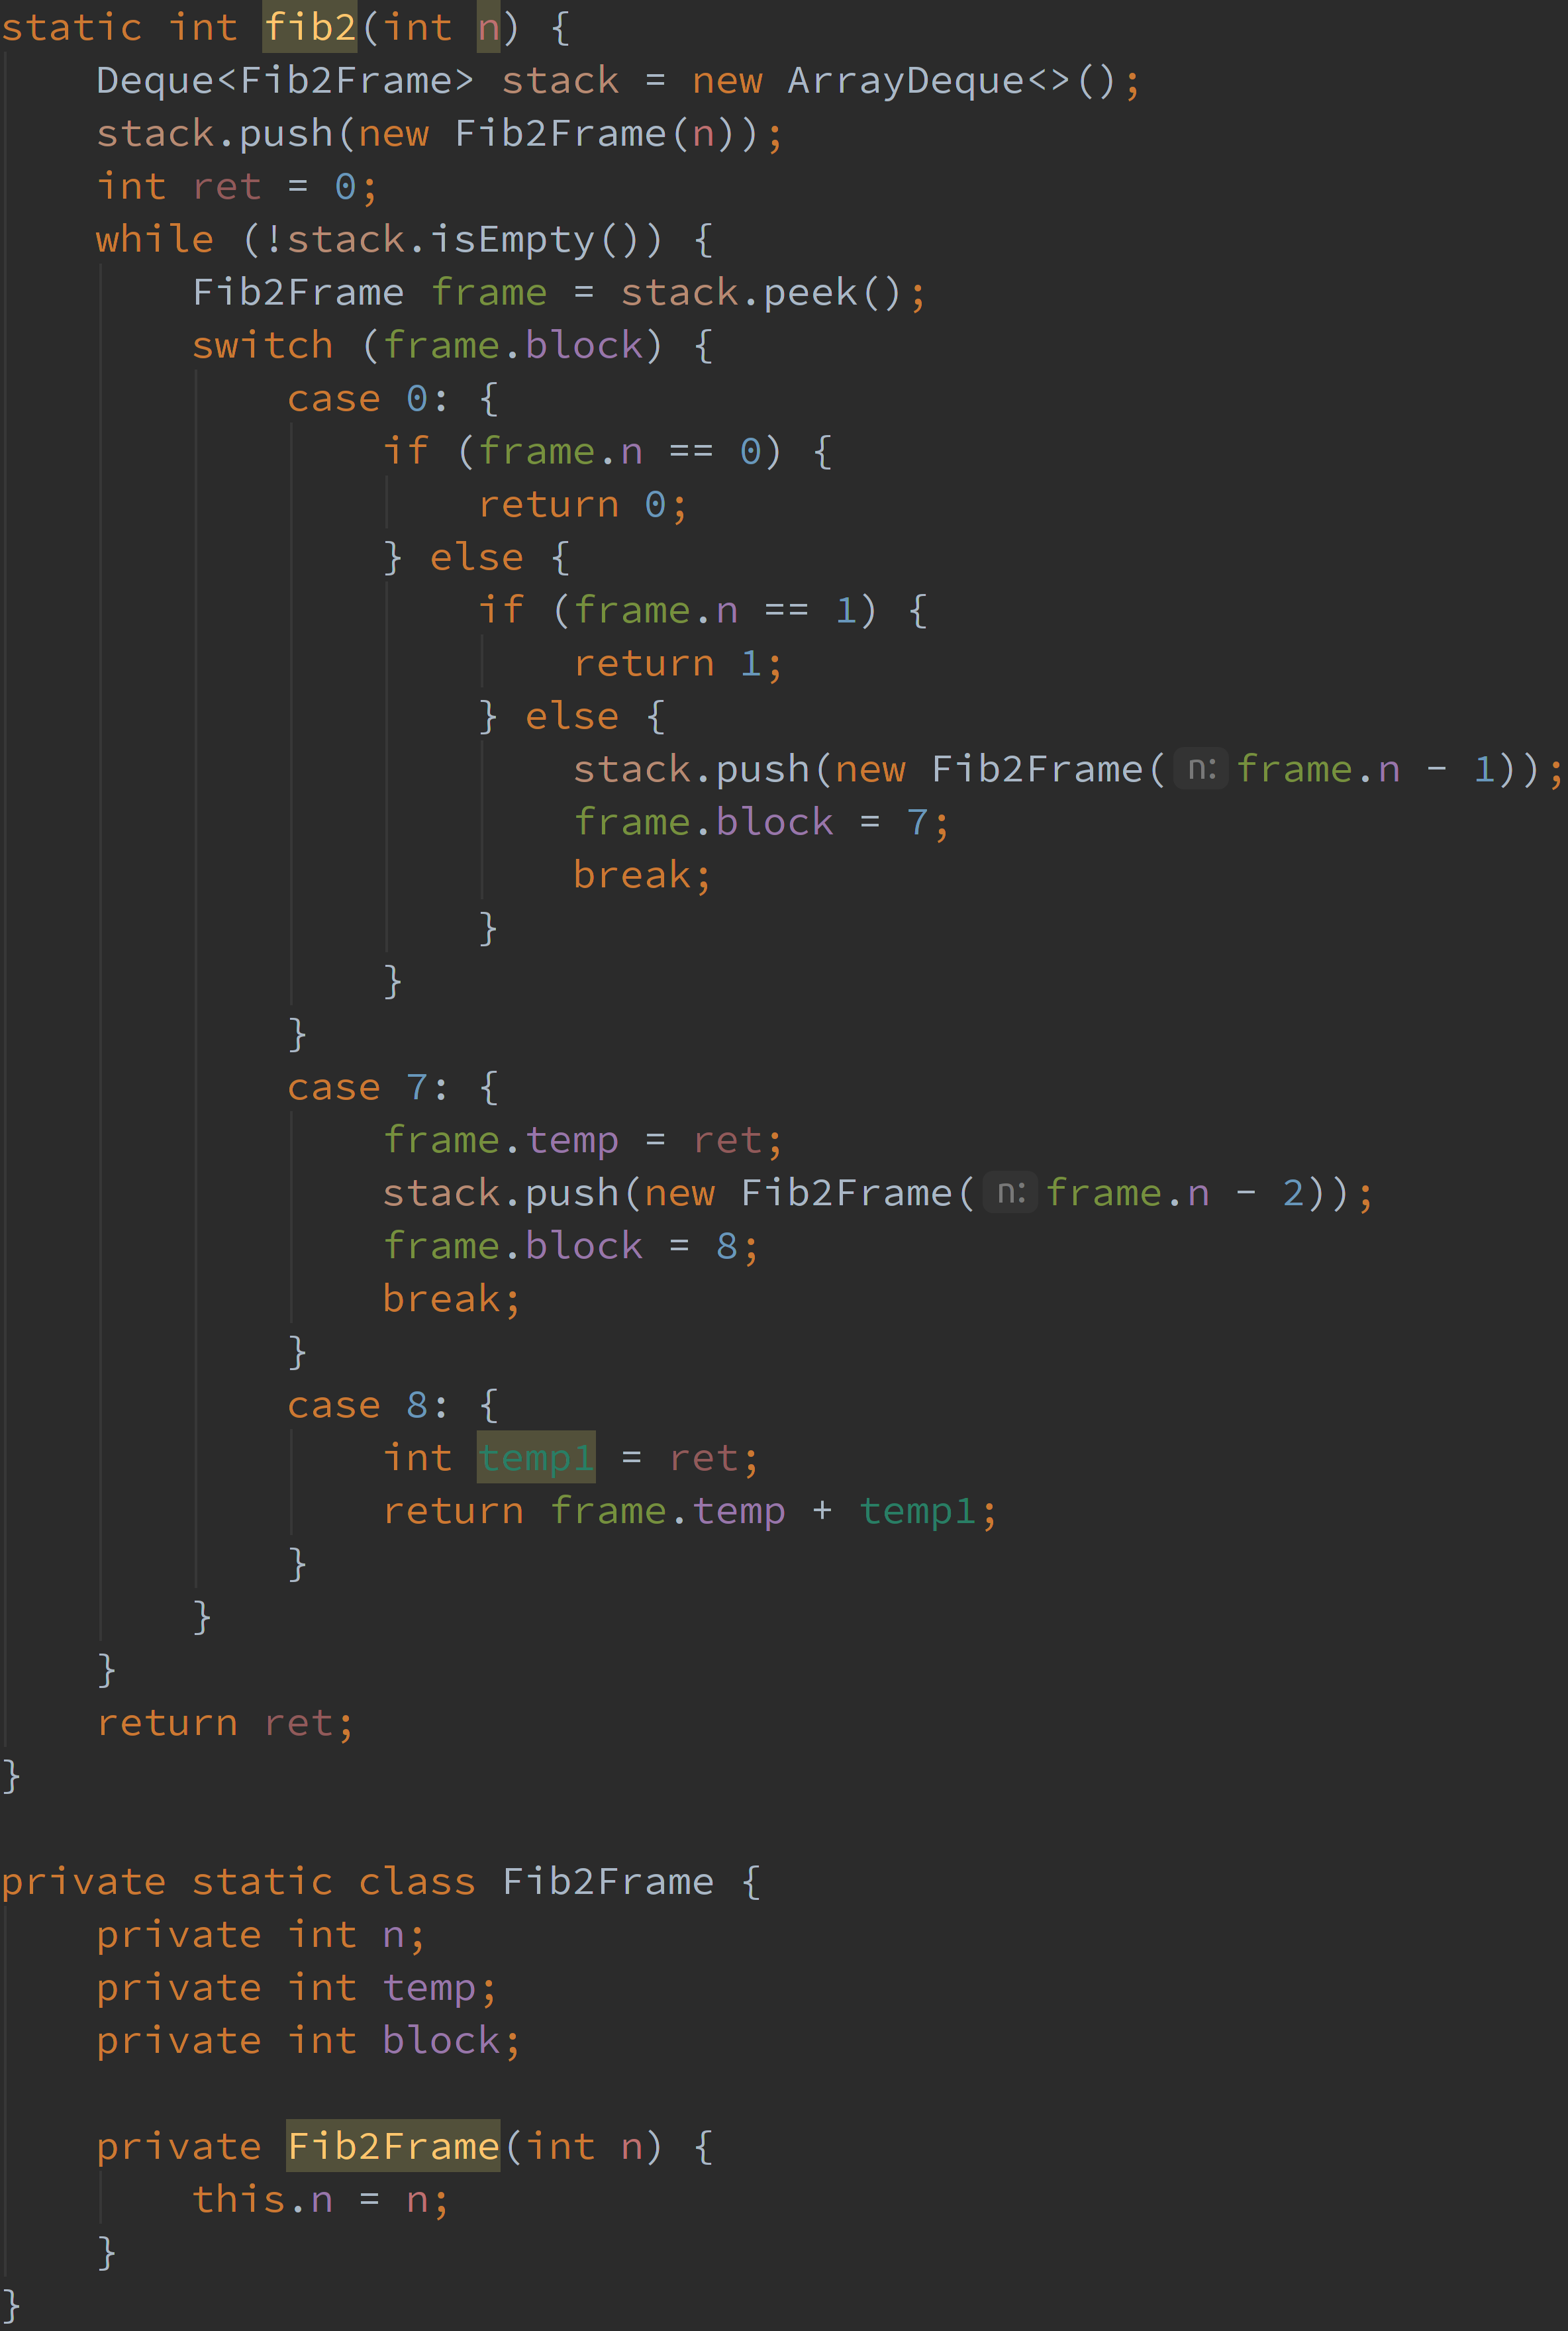
\includegraphics[height=4.4in]{src/img/inline-blocks-after-44.png}
        \caption{After}
    \end{subfigure}%
    }\\
    \caption{Inlining blocks \label{img:inline-blocks}}
\end{figure}